\section{Fluxo de avaliação de vida à fadiga em dutos em vão-livre}\label{chap:workflow}


Baseado nos estudos e oficinas realizados para o desenvolvimento deste trabalho. Pôde-se estabelecer que a análise de vida a fadiga em dutos em vão-livre compreende o fluxograma apresentado na \autoref{fig:fluxograma}.

\begin{figure}[!ht]
    \centering
    \caption{Fluxo de avaliação de vida à fadiga em dutos em vão-livre.}\label{fig:fluxograma}
    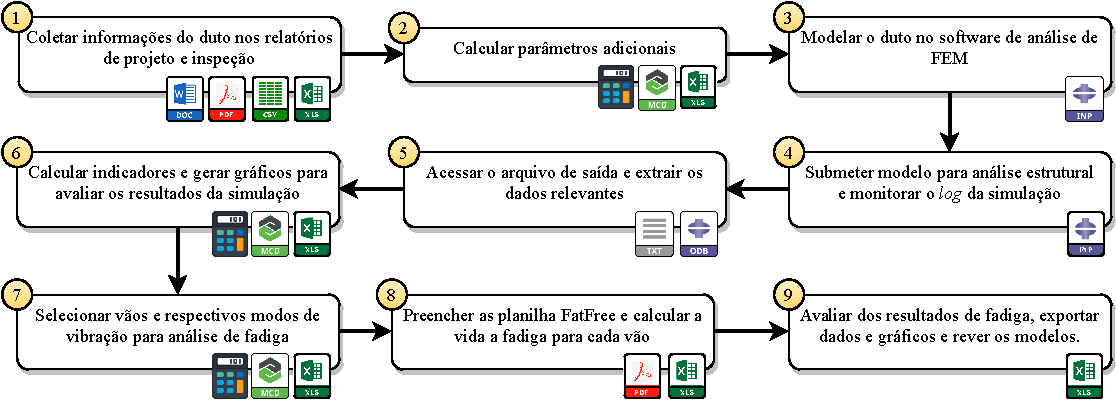
\includegraphics[width=\textwidth]{imagens/fluxograma.pdf}
    \fonte{Autor (2020)}
\end{figure}

A seguir, uma breve descrição de cada item:

\begin{enumerate}[label=(\arabic*)]
    \item Nesta etapa, o profissional reúne as informações básicas para construção dos modelos e outros dados usados em cálculos posteriores. Citadamente, temos aqui: as cotas do perfil do duto e batimetria obtidas na inspeção, geometria e propriedades dos materiais das camadas que compõem sessão do duto, parâmetros do solo, coeficientes de segurança e outras constantes físicas, posição e tipos de suportes ao longo do duto. Essa tarefa envole olhar uma série de documentos (\texttt{.doc}, \texttt{.pdf}, etc) em busca desses valores, dispostos de forma não estruturada. Quando estruturados, em forma de arquivos CSV ou planilhas, por exemplo, é necessário ainda manipular esses dados a fim de extrair somente a informação necessária e/ou convertê-las no formato apropriado. Um exemplo disso são os dados de batimetria, que precisam convertidos nas coordenadas dos nós de uma malha de elementos finitos no formato de um arquivo \texttt{.inp}. -- no caso do \abaqus. De posse desses dados, pode-se então, iniciar a fase de pré-processamento.
    \item Uma vez que nem todos os dados a serem utilizados estão de acordo com as especificações dos softwares a serem empregados nas análises numéricas, ainda é necessários manipular alguns desses valores, seja calculando constantes ou convertendo unidades. Para isso, geralmente utiliza-se softwares de planilhas e/ou folhas de cálculos (Microsft Excel, MathCad, Maple, etc.). Esta etapa inicia o pré-processamento dos dados.
    \item Com todos os dados em mãos, é necessário transformá-los em um modelo no software de elementos finitos, via interação com mouse e teclado (GUI\footnote{\textit{}{Graphical User Interface}}: interface de usuário gráfica), ou criando arquivos de entrada. Embora a reutilização de arquivos de entrada previamente criados facilite esse tarefa, nem todos os trechos desses arquivos são suficientes ou podem ser reaproveitados. Estas limitações são frequentes em trechos do arquivo que precisam ser repetidos a depender da quantidade de certas entidades no modelo -- suportes, por exemplo. Ao fim desta etapa, encerra-se o pré-processamento dos dados.
    \item Por mais simples que seja submeter o modelo para análise na maioria dos softwares de análise de elementos (alguns cliques via GUI, ou um comando via CLI, as análises costumam levar horas e envolver execuções sucessivas a fim de realizar intervenções no modelo que não podem ser modeladas previamente. Dessa forma, torna-se necessário o monitoramento do progresso da simulação. Esta etapa compreende a primeira parte do processamento propriamente dito.
    \item Uma vez concluída a simulação Análise de Elementos Finitos (FEA, em inglês), é necessário analisar os resultados antes do pós-processamento. Por vezes, é preciso extrair os resultados que estão armazenados em arquivos proprietários (como \texttt{.odb}, no caso do \abaqus), utilizando as funcionalidades das ferramentas dos próprios pacotes de software de elementos finitos para isso. Esta tarefa, geralmente feita via GUI, costuma ser repetitiva e pode levar de alguns minutos ou horas. Esta etapa inicia parte do pós-processamento da FEA.
    \item De posse dos resultados em formatos acessíveis a outros software (MS Excel e MathCad, por exemplo), é necessário calcular (e muitas vezes visualizar em gráficos) alguns indicadores a fim de avaliar a validade dos resultados. Embora poderosos, estes softwares ainda carecem de gráficos mais interativos, como possibilidades de ampliar e transladar os gráficos com o mouse. Esta etapa encerra o pós-processamento da FEA.
    \item Na metodologia presente na \dnvf105 -- que será abordada adiante no \autoref{sec:multimode} -- o cálculo de fadiga é baseada em modelos de resposta, portanto, é necessário calcular a resposta de cada modo para as várias condições de carregamento ambiental, o que a torna impraticável sem automação. Para solucionar este problema, foi criada a \fatfree, uma planilha de cálculo comercial que realiza estas operações. No entanto, dentre as dezenas de modos obtidos por solução modal na FEA costumam aparecer modos espúrios. Dessa forma, antes de realizar a análise na \fatfree, é necessário escolher dentre os modos de vibração obtidos na simulação numérica aqueles que mais contribuem para fadiga. Esta tarefa pode ser feita via inspeção visual, observando a forma dos modos, mas é uma prática mas pouco precisa e subjetiva.
    \item Uma vez selecionados os modos a serem usados para cálculo de fadiga, é necessário o preenchimento da planilha com os dados de deflexão normalizada de cada modos, o que consiste em algumas centenas de valores. Além disso, é necessário preencher muitas outras informações referentes geometria e propriedades dos materiais da sessão do duto, parâmetros do solo, coeficientes de segurança e condições de carregamento em várias páginas diferentes. Com todos os dados preenchidos e opções selecionadas nos controles da planilha, pode-se apertar o botão que calcula os resultados de fadiga.
    \item Finalmente, os dados de fadiga pode ser analisados e exportados para outras ferramentas a fim de gerar relatórios.
\end{enumerate}